%%%%%%%%%%%%%%%%%%%%%%%%%%%%%%%%%%%%%%%%%%%%%%%%%%%%%%%%%%%%%%%%%%%%%%%%%%%%%%%
% Overview of the methodology to be used.
% \newpage

\begin{figure}
    \centering
    \graphicspath{ {../schemas/methodology/} }
    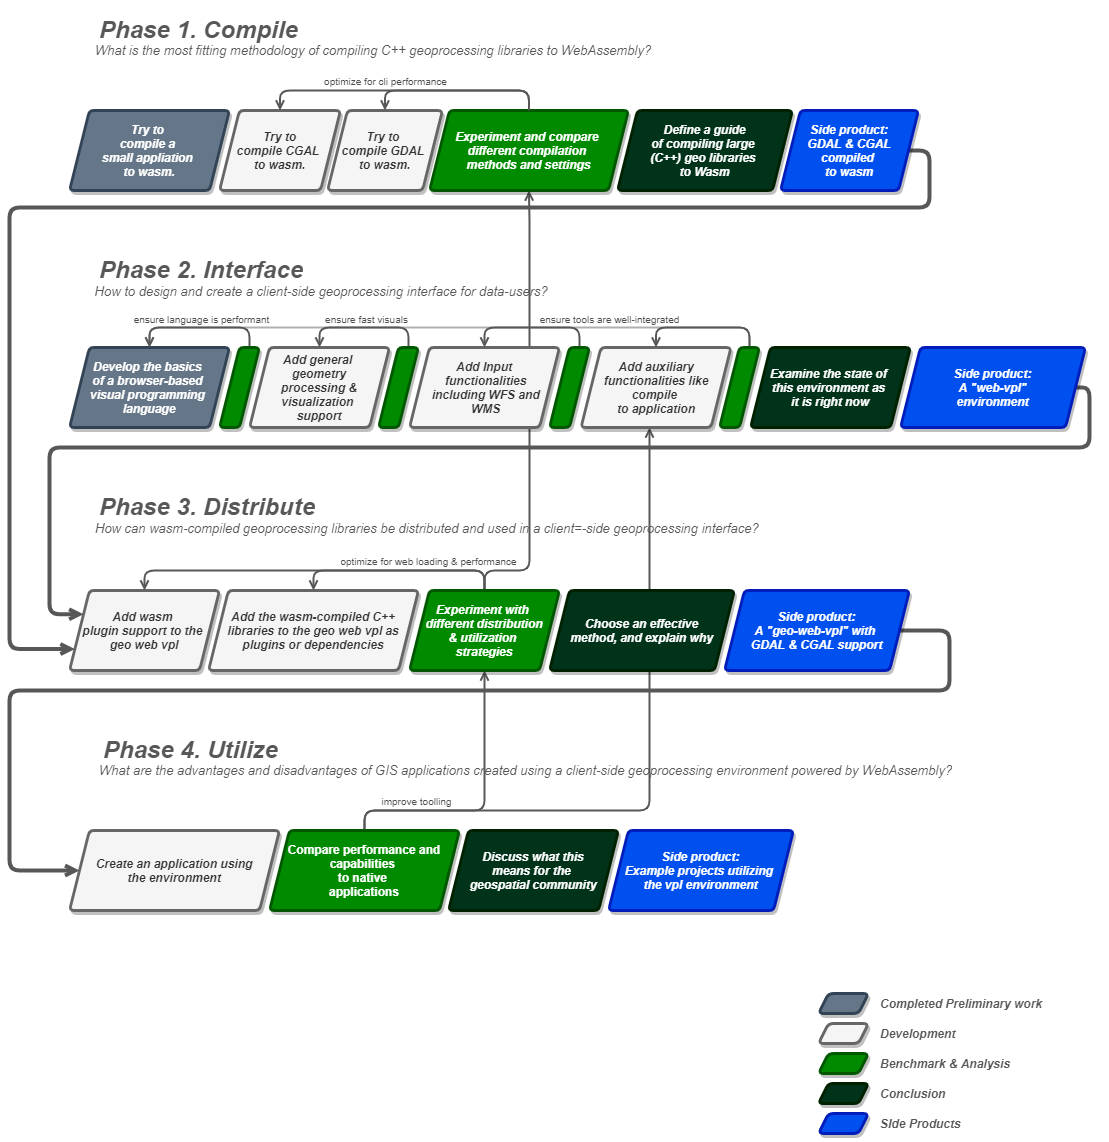
\includegraphics[width=14cm]{method.png}
    \caption{Methodology schema}
    \label{fig:method}
\end{figure}

\section{Methodology}

This brings us to the methodology of this study. To find answers to the main research question, this study will be divided into four phases, each matching a certain sub-research question. A phase has two goals. The primary goal is to answer its corresponding research question, and to cover the process towards this answer. The secondary goal is to describe the development of the software required to form this answer. This software can be seen as a "side product", and will be a required starting point to answer subsequent questions, as well as a vital component of the use-case application. 

\reffig{fig:method} offers an overview of the full methodology. The schema acts as a general guide, and is subject to change, based on the obstacles encountered during the study. Please note this causality between the different phases, represented by thick arrows. The Compile and Interface phases can be executed in parallel, and require no particular order. The Synthesize and Utilize phases phases depend on side products from phases before it. 

The methodology used can be characterized as both incremental and iterative. Its incremental nature means that every phase, and every step within a phase, will produce meaningful in-between products \& results. This ensures the study will be insightful, even in the case the full scope of this study might become unfeasible. It is also vital for making the methodology iterative. 

The study's iterative nature, represented by the cyclic paths within \reffig{fig:method}, means that analysis and benchmarks will not be postponed until the end of the study, and will instead be an intricate part of each step. This makes sure obstacles are discovered early, and the trajectory of the study can be adjusted dynamically.  

Every phase contains a number of development \& analysis steps. The reasoning behind these steps, are covered by the following sub-chapters.  

%%%%%%%%%%%%%%%%%%%%%%%%%%%%%%%%%%%%%%%%%%%%%%%%%%%%%%%%%%%%%%%%%%%%%%%%%%%%%%%

\subsection{Phase 1: Compile}

% not as easy 
% The study starts out with the assumption that WebAssembly must be utilized to properly compile and run existing geoprocessing libraries in a browser. This might not be as easy as using normal compilers, based on the experience gained by preliminary work (See \autoref{sec:preliminary-wasm}). WebAssembly is containerized and makes no assumptions about its source language \cite{haas_bringing_2017}, making aspects such as an SDK, sub-dependencies called using environment variables, and IO (file reading and writing) possible obstacles. These aspects might be solved by using or writing wrapper libraries and using file system workarounds, as proposed by \cite{jangda_not_2019}. 

% question & steps to answer
The first sub-research question is dedicated to overcoming Obstacle 1, as well the related works on \ac{wasm}. It goes: \textbf{"What is the most fitting methodology of compiling C++ geoprocessing libraries to WebAssembly?"}.
We specify ourselves to C++, since this seems to be the language of choice for almost all well established geoprocessing libraries. 
'Fitting' in this context refers to the specific requirements posed by geoprocessing libraries. 
The libraries are complex and sizable, and the geodata used as input even more so. 
This means special attention will be given to these aspects. 
Standard compiler effectiveness criteria, such as portability (smallest file size), and performance, will also be considerations during the assessment of methodologies.  

While the question poses to find the \textit{best} compilation method, if it turns out that only one method makes it possible to compile sizable geo-libraries, this phase will nonetheless regard itself as successful. The question will have to be rephrased in that case. 

% performance
\subsubsection*{Performance}
The performance benefit of WebAssembly is an important component of why WebAssembly might be beneficial for client-side geoprocessing. As such, this phase is interested in confirming whether this is the case for geoprocessing applications. Once a sufficient compilation method is found, individual functions of geoprocessing libraries will be benchmarked using three different methods: 

\begin{itemize}
    \item Compiled and run as native binary (g++), 
    \item Compiled to wasm, run natively (WASI),
    \item Compiled to asm.js, run natively (NODE.js),
\end{itemize}

% why cgal & GDAL
\subsubsection*{Test Cases}
CGAL \& GDAL will be used as examples of "C++ geoprocessing libraries" for this phase. For one, these libraries are well established and relevant to geoprocessing as a whole. Many other geo-libraries depend on them. Moreover, they are properly sizable and complex, making it highly likely the problems described earlier will be encountered. We could choose "easier" libraries, but this will not be representative of most C++ geoprocessing libraries. And, while CGAL, and GDAL will be this phase's primary subject, the answer of this research question aims to be a guide applicable to all geoprocessing libraries. 

%%%%%%%%%%%%%%%%%%%%%%%%%%%%%%%%%%%%%%%%%%%%%%%%%%%%%%%%%%%%%%%%%%%%%%%%%%%%%%%
\newpage
\subsection{Phase 2: Interface}

Phase 2 is dedicated to overcoming Obstacle 2, together with the related works on the geoweb (See \refsec{sec:geoweb}). Phase 2 seeks to not only make geoprocessing runnable, but actually usable, and usable to a wider audience than just geodata processing experts, called "data-users". This quest is posed using the research question: \textit{How to design and create a client-side geoprocessing interface for data-users?}. 

Phase 2 will primarily be about implementing the foundations of the use-case application 'GeoFront'. None of the existing web-based \ac{vpl}'s were deemed acceptable for the scope of this study, so the application will have to be created from scratch. 
The application will be created using JavaScript, or its type-save equivalent TypeScript. 
A choice can be made to write the whole environment as a native application which then, as a whole, can be published to the web using WebAssembly. 
This would probably be the most performant. 
However, referring back to the FAIR principles of \cite{mark_d_wilkinson_fair_2016}, this would be detrimental to the concept of Interoperability and Reusability. 
We wish the environment to contain small, standalone components which could be useful in of themselves. 
For example, users might want to integrate a geodata process on their own website without the full \ac{gui} attached.

The modern web contains many technologies we can possibly use to facilitate all required features. WebGL offers the ability to efficiently visualize 3D data. The 2d canvas API and SVG's can be used to visualize 2D data. HTML can be used to build the interface.

\subsubsection*{Steps}

Just like the entire study, the development trajectory during phase 2 will be done incrementally, ensuring results can be shown during all steps of the development. 
The first step of the phase will consist of creating the basics of the \ac{gui} itself. a basic \ac{vpl} will be created which can only process boolean statements. The second step adds types, geometry, and the visualization of this geometry in 3D, as well as textures / images in 2d. The third step will add geospatial data support, like Web Feature Services, Web Map Services, and coordinate reference systems.  

%%%%%%%%%%%%%%%%%%%%%%%%%%%%%%%%%%%%%%%%%%%%%%%%%%%%%%%%%%%%%%%%%%%%%%%%%%%%%%%

\subsection{Phase 3: Distribute}

% performant and sharable geoprocessing
% portability


The third phase is characterized by harmonizing the results of Phase 1 and 2. 
The related works pointed out that WebAssembly can only truly be tested within a realistic use-case scenario, So this Phase intends to do just that.
The research question goes: \textit{What is the best way of distributing wasm-compiled geoprocessing libraries, in order to use them within a client-side geoprocessing interface?}. 
This phase can be seen as a continuation of phase 1, but where the compilation research of phase 1 limits itself to native, CLI usage of WebAssembly, this phase introduces the web, and the developed interface during phase 2 as new factors to this research. Given this as the desired way of processing geodata, how can WebAssembly facilitate these desires? 

This will result in new benchmarks, and new analyses, now including factors like client-side (down)load times, compilation, and utilization. Answers will have to be given to questions such as \textit{Where do the wasm-compiled libraries live?} and \textit{ how are they cached? }.

One of the hypothetical obstacles during this phase is that an entire geoprocessing libraries will have to be downloaded, even if the user desires only a single function. A solution to this problem is to increase granularity, and split up the C++ libraries to several smaller ones, maybe even one wasm binary per function or class. This would be accompanied by WebAssemblies ability to accept \ac{wasm} dependencies at the time it is loaded into memory. 




%%%%%%%%%%%%%%%%%%%%%%%%%%%%%%%%%%%%%%%%%%%%%%%%%%%%%%%%%%%%%%%%%%%%%%%%%%%%%%%
\subsection{Phase 4: Utilize}

Finally, When the VPL contains all tools necessary to be used to properly process geodata, a final assessment can be made by using the environment to serve as an application. this assessment will try to overcome Obstacle 3 by posing the question: \textit{What are the advantages and disadvantages of GIS applications created using a client-side geoprocessing environment powered by WebAssembly?}. This question requires a native but comparable GIS application to test this against.  

I hypothesize that applications equipped with client-side geoprocessing open up a whole range of new possibilities posing both academic \& commercial benefits. 
I intent to discuss these aspects of the study during this phase. 


% Three different 
% and these same applications will be created using the prototype web-VPL. 
% These two methods will then be compared on usability aspects and performance.   

% ## 5.3 Case Study

\subsubsection*{Case Study}

This is a sketch of an application which could be created if the use-case application performs as intended. A series of steps \& geoprocessing operations are given to give an impression of the complexity of such an application.

\begin{lstlisting}
# Demo Application: On Demand Isocurves Generator

# Input: 
- Point Cloud

# Output
- Line Curves / .png render of line curves

# Steps: 
- Load ahn3 point-cloud 
  (WFS Input Widget | WFS Preview Widget)
- Visualize point cloud on top of base map of the netherlands 
  (WMS Input Widget | WMS > Preview Widget)
- Only select terrain points (list filter Operation)
- Construct a 2d polygon by clicking points on a map 
  (Polygon Input Widget)
- Select Area of interest using a 2d polygon 
  (Boundary Include Operation)
- Triangulate point cloud with a certain resolution 
  (Triangulate Operation)
- Intersect the mesh surface with a series of planes 
  (Isocurves from Mesh Operation)
- Preview data 
  (MultiLine Preview Widget)
- Export data 
  (MultiLine export Widget)
\end{lstlisting}
